\scalebox{0.8}{ % Adjust scale if needed
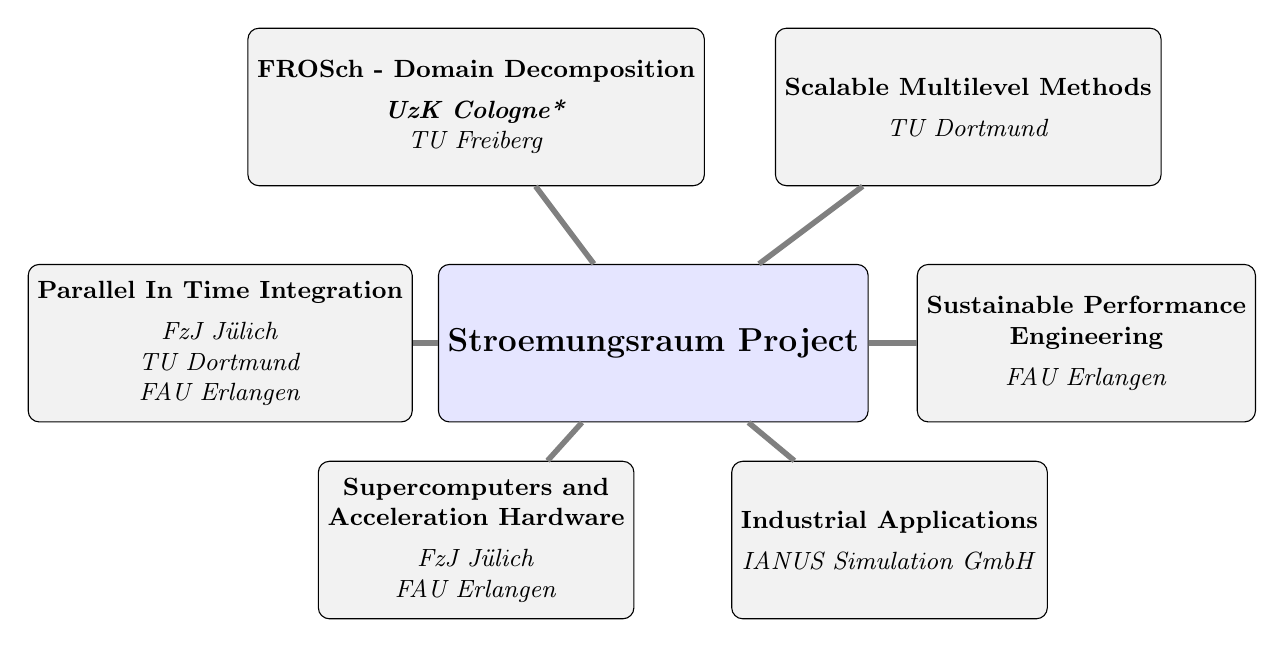
\begin{tikzpicture}[
  % Removed "mindmap" as it applies specific styling that's hard to override
  every node/.style={
    rectangle,
    rounded corners,
    minimum width=2cm,
    minimum height=2cm,
    align=center,
    font=\small,
    text=black,
    draw=black,
    fill=gray!10
  },
  root concept/.style={
    fill=blue!10,
    font=\bfseries\large,
    text=black,
    minimum width=3cm
  },
  % Custom edge style
  conn/.style={
    draw=black!50,
    line width=2pt,
    solid
  },
]
\node[root concept] (root) {Stroemungsraum Project};

% Create child nodes with explicit positioning and manual edges
\node[xshift=5.5cm, yshift=0cm] (n1) {\bf{Sustainable Performance}\\\bf{Engineering}\\[1ex] \textit{FAU Erlangen}};
\node[xshift=4cm, yshift=3cm] (n2) {\bf{Scalable Multilevel Methods}\\[1ex] \textit{TU Dortmund}};
\node[xshift=-2.25cm, yshift=3cm] (n3) {\bf{FROSch - Domain Decomposition}\\[1ex]\textit{\textbf{UzK Cologne*}}\\ \textit{TU Freiberg}};
    \node[xshift=-5.5cm, yshift=0cm] (n4) {\bf{Parallel In Time Integration}\\[1ex] \textit{FzJ Jülich}\\ \textit{TU Dortmund}\\ \textit{FAU Erlangen}};
\node[xshift=-2.25cm, yshift=-2.5cm] (n5) {\bf{Supercomputers and}\\\bf{Acceleration Hardware}\\[1ex] \textit{FzJ Jülich}\\\textit{FAU Erlangen}};
    \node[xshift=3cm, yshift=-2.5cm] (n6) {\bf{Industrial Applications}\\[1ex] \textit{IANUS Simulation GmbH}};
%
% % Draw thin connections
\draw[conn] (root) -- (n1);
\draw[conn] (root) -- (n2);
\draw[conn] (root) -- (n3);
\draw[conn] (root) -- (n4);
\draw[conn] (root) -- (n5);
\draw[conn] (root) -- (n6);
\end{tikzpicture}
}
